% uncertainty_plane: support s (effective views) against agreement rho_hat.
% Regions follow usplat/vmf_field.py defaults: tau_min = 3 views, robust set rho_hat >= 0.6 and
% not flagged changed. Change is a test over time (Sec. change), so it is not a region here.
% The curves are closed-form expectations for equal full-weight views (omega = 1, so s = number
% of views) whose view means u_v have unit length and mean E[u] of length rho:
%   ||R||/W_1           : sqrt(rho^2 + (1 - rho^2)/s)             (root mean square), rho = 0.35
%   ||R||/(W_1 + c_0)   : sqrt(rho^2 + (1 - rho^2)/s) * s/(s + 1)  (c_0 = 1),          rho = 0.90
%   rho_hat             : E[rho_hat^2] = rho^2 before the clamp (unbiased), drawn at rho for s >= tau_min
%                         (the clamp and the sqrt leave a small bias; mean stays close to rho)
% Monte Carlo check (d = 64, 20000 trials): the two curves match the simulated means within 0.001;
% E[rho_hat] = 0.334 (rho = 0.35, 3 views), 0.349 (12 views), 0.900 (rho = 0.90).
% They illustrate the bias of each estimator; they are not measured data.
% Build (from papers/): tectonic figs/uncertainty_plane.tex. Natural width ~ \columnwidth (3.4 in).
\documentclass[tikz,border=2pt]{standalone}
\usepackage{amsmath,amssymb}
\usetikzlibrary{arrows.meta,calc}
\newcommand{\R}{\mathbf{R}}

\begin{document}
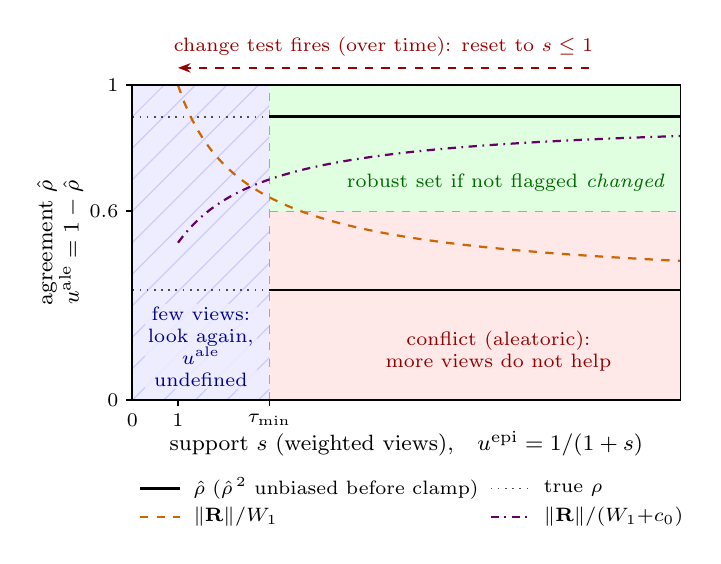
\begin{tikzpicture}[font=\footnotesize, line width=0.6pt]

% ---- geometry: x = \sx * s (views), y = \sy * value ----
\def\sx{0.58}   % cm per view
\def\sy{4.00}   % cm per unit of agreement
\def\smax{12}   % right end of the s axis (views)
\def\taumin{3}  % tau_min (views)
\def\rrob{0.6}  % agreement threshold of the robust set
\def\rlo{0.35}  % example: conflicting Gaussian (true rho)
\def\rhi{0.90}  % example: consistent Gaussian (true rho)
\pgfmathsetmacro{\X}{\sx*\smax}
\pgfmathsetmacro{\xt}{\sx*\taumin}
\pgfmathsetmacro{\yr}{\sy*\rrob}
\pgfmathsetmacro{\ylo}{\sy*\rlo}
\pgfmathsetmacro{\yhi}{\sy*\rhi}

% ---- regions ----
\fill[blue!7]   (0,0) rectangle (\xt,\sy);
\fill[green!12] (\xt,\yr) rectangle (\X,\sy);
\fill[red!9]    (\xt,0) rectangle (\X,\yr);
\begin{scope}
  \clip (0,0) rectangle (\xt,\sy);
  \foreach \s in {-4.0,-3.6,...,1.6}
    \draw[blue!20, line width=0.4pt] (\s,0) -- (\s+4.0,\sy);
\end{scope}
\draw[gray!70, dashed, line width=0.5pt] (\xt,0) -- (\xt,\sy);
\draw[gray!70, dashed, line width=0.5pt] (\xt,\yr) -- (\X,\yr);

% ---- true agreement of the two example Gaussians (dotted) ----
\draw[gray!60!black, dotted, line width=0.6pt] (0,\ylo) -- (\X,\ylo);
\draw[gray!60!black, dotted, line width=0.6pt] (0,\yhi) -- (\X,\yhi);

% ---- mean resultant length ||R||/W_1 of the conflicting Gaussian: biased up ----
\draw[orange!80!black, dashed, line width=0.8pt]
  plot[domain=1:\smax, samples=80] ({\sx*\x}, {\sy*sqrt(\rlo*\rlo + (1-\rlo*\rlo)/\x)});
% ---- prior-shrunk agreement ||R||/(W_1+c_0) of the consistent Gaussian: biased down ----
\draw[violet!80!black, dash dot, line width=0.8pt]
  plot[domain=1:\smax, samples=80] ({\sx*\x}, {\sy*sqrt(\rhi*\rhi + (1-\rhi*\rhi)/\x)*\x/(\x+1)});
% ---- rho_hat: unbiased, defined from tau_min on ----
\draw[black, line width=1.0pt] (\xt,\ylo) -- (\X,\ylo);
\draw[black, line width=1.0pt] (\xt,\yhi) -- (\X,\yhi);

% ---- region labels ----
\node[align=center, text=blue!55!black, font=\scriptsize, inner sep=1pt, fill=blue!7,
      fill opacity=0.85, text opacity=1] at (0.5*\xt,0.68)
  {few views:\\ look again,\\ $u^{\mathrm{ale}}$\\ undefined};
\node[align=center, text=green!40!black, font=\scriptsize] at ({0.5*(\xt+\X)+0.40},{\yr+0.36})
  {robust set if not flagged \emph{changed}};
\node[align=center, text=red!55!black, font=\scriptsize] at ({0.5*(\xt+\X)+0.3},0.62)
  {conflict (aleatoric):\\ more views do not help};

% ---- change: a test over time, drawn above the plane ----
\draw[red!60!black, dashed, line width=0.6pt, -{Stealth[length=1.6mm]}]
  (\sx*10,\sy+0.22) -- (\sx*1,\sy+0.22);
\node[font=\scriptsize, text=red!60!black, anchor=south] at ({\sx*5.5},\sy+0.24)
  {change test fires (over time): reset to $s\le1$};

% ---- axes ----
\draw[black, line width=0.6pt] (0,0) rectangle (\X,\sy);
\foreach \s/\l in {1/{$1$}, \taumin/{$\tau_{\min}$}} {
  \draw (\sx*\s,0) -- (\sx*\s,-0.08);
  \node[font=\scriptsize, below] at (\sx*\s,-0.05) {\l};
}
\node[font=\scriptsize, below] at (0,-0.05) {$0$};
\foreach \v in {0,0.6,1} {
  \draw (0,\sy*\v) -- (-0.08,\sy*\v);
  \node[font=\scriptsize, left] at (-0.05,\sy*\v) {$\v$};
}
\node at (\X/2,-0.55) {support $s$ (weighted views),\quad $u^{\mathrm{epi}}=1/(1+s)$};
\node[rotate=90, align=center] at (-0.92,\sy/2) {agreement $\hat\rho$\\ $u^{\mathrm{ale}}=1-\hat\rho$};

% ---- legend ----
\begin{scope}[shift={(0.1,-1.12)}, font=\scriptsize]
  \draw[black, line width=1.0pt] (0,0) -- (0.5,0);
  \node[anchor=west] at (0.55,0) {$\hat\rho$ ($\hat\rho^{\,2}$ unbiased before clamp)};
  \draw[gray!60!black, dotted, line width=0.6pt] (4.45,0) -- (4.95,0);
  \node[anchor=west] at (5.00,0) {true $\rho$};
  \draw[orange!80!black, dashed, line width=0.8pt] (0,-0.36) -- (0.5,-0.36);
  \node[anchor=west] at (0.55,-0.36) {$\lVert\R\rVert/W_1$};
  \draw[violet!80!black, dash dot, line width=0.8pt] (4.45,-0.36) -- (4.95,-0.36);
  \node[anchor=west] at (5.00,-0.36) {$\lVert\R\rVert/(W_1{+}c_0)$};
\end{scope}
\end{tikzpicture}
\end{document}
